\documentclass[twocolumn]{article}
\usepackage[utf8]{inputenc}
\usepackage[top=1in]{geometry}
\usepackage{graphicx}
\usepackage{booktabs}
\usepackage{amsmath,amssymb}
\usepackage{xcolor}
\usepackage{multirow}
% Calligraphic fonts
\newcommand{\calA}{{\cal A}}
\newcommand{\calB}{{\cal B}}
\newcommand{\calC}{{\cal C}}
\newcommand{\calD}{{\cal D}}
\newcommand{\calE}{{\cal E}}
\newcommand{\calF}{{\cal F}}
\newcommand{\calG}{{\cal G}}
\newcommand{\calH}{{\cal H}}
\newcommand{\calI}{{\cal I}}
\newcommand{\calJ}{{\cal J}}
\newcommand{\calK}{{\cal K}}
\newcommand{\calL}{{\cal L}}
\newcommand{\calM}{{\cal M}}
\newcommand{\calN}{{\cal N}}
\newcommand{\calO}{{\cal O}}
\newcommand{\calP}{{\cal P}}
\newcommand{\calQ}{{\cal Q}}
\newcommand{\calR}{{\cal R}}
\newcommand{\calS}{{\cal S}}
\newcommand{\calT}{{\cal T}}
\newcommand{\calU}{{\cal U}}
\newcommand{\calV}{{\cal V}}
\newcommand{\calW}{{\cal W}}
\newcommand{\calX}{{\cal X}}
\newcommand{\calY}{{\cal Y}}
\newcommand{\calZ}{{\cal Z}}

% Sets:
\newcommand{\setA}{\textsf{A}}
\newcommand{\setB}{\textsf{B}}
\newcommand{\setC}{\textsf{C}}
\newcommand{\setD}{\textsf{D}}
\newcommand{\setE}{\textsf{E}}
\newcommand{\setF}{\textsf{F}}
\newcommand{\setG}{\textsf{G}}
\newcommand{\setH}{\textsf{H}}
\newcommand{\setI}{\textsf{I}}
\newcommand{\setJ}{\textsf{J}}
\newcommand{\setK}{\textsf{K}}
\newcommand{\setL}{\textsf{L}}
\newcommand{\setM}{\textsf{M}}
\newcommand{\setN}{\textsf{N}}
\newcommand{\setO}{\textsf{O}}
\newcommand{\setP}{\textsf{P}}
\newcommand{\setQ}{\textsf{Q}}
\newcommand{\setR}{\textsf{R}}
\newcommand{\setS}{\textsf{S}}
\newcommand{\setT}{\textsf{T}}
\newcommand{\setU}{\textsf{U}}
\newcommand{\setV}{\textsf{V}}
\newcommand{\setW}{\textsf{W}}
\newcommand{\setX}{\textsf{X}}
\newcommand{\setY}{\textsf{Y}}
\newcommand{\setZ}{\textsf{Z}}

% Vectors
\newcommand{\bfa}{\mathbf{a}}
\newcommand{\bfb}{\mathbf{b}}
\newcommand{\bfc}{\mathbf{c}}
\newcommand{\bfd}{\mathbf{d}}
\newcommand{\bfe}{\mathbf{e}}
\newcommand{\bff}{\mathbf{f}}
\newcommand{\bfg}{\mathbf{g}}
\newcommand{\bfh}{\mathbf{h}}
\newcommand{\bfi}{\mathbf{i}}
\newcommand{\bfj}{\mathbf{j}}
\newcommand{\bfk}{\mathbf{k}}
\newcommand{\bfl}{\mathbf{l}}
\newcommand{\bfm}{\mathbf{m}}
\newcommand{\bfn}{\mathbf{n}}
\newcommand{\bfo}{\mathbf{o}}
\newcommand{\bfp}{\mathbf{p}}
\newcommand{\bfq}{\mathbf{q}}
\newcommand{\bfr}{\mathbf{r}}
\newcommand{\bfs}{\mathbf{s}}
\newcommand{\bft}{\mathbf{t}}
\newcommand{\bfu}{\mathbf{u}}
\newcommand{\bfv}{\mathbf{v}}
\newcommand{\bfw}{\mathbf{w}}
\newcommand{\bfx}{\mathbf{x}}
\newcommand{\bfy}{\mathbf{y}}
\newcommand{\bfz}{\mathbf{z}}


\newcommand{\bfalpha}{\boldsymbol{\alpha}}
\newcommand{\bfbeta}{\boldsymbol{\beta}}
\newcommand{\bfgamma}{\boldsymbol{\gamma}}
\newcommand{\bfdelta}{\boldsymbol{\delta}}
\newcommand{\bfepsilon}{\boldsymbol{\epsilon}}
\newcommand{\bfzeta}{\boldsymbol{\zeta}}
\newcommand{\bfeta}{\boldsymbol{\eta}}
\newcommand{\bftheta}{\boldsymbol{\theta}}
\newcommand{\bfiota}{\boldsymbol{\iota}}
\newcommand{\bfkappa}{\boldsymbol{\kappa}}
\newcommand{\bflambda}{\boldsymbol{\lambda}}
\newcommand{\bfmu}{\boldsymbol{\mu}}
\newcommand{\bfnu}{\boldsymbol{\nu}}
\newcommand{\bfomicron}{\boldsymbol{\omicron}}
\newcommand{\bfpi}{\boldsymbol{\pi}}
\newcommand{\bfrho}{\boldsymbol{\rho}}
\newcommand{\bfsigma}{\boldsymbol{\sigma}}
\newcommand{\bftau}{\boldsymbol{\tau}}
\newcommand{\bfupsilon}{\boldsymbol{\upsilon}}
\newcommand{\bfphi}{\boldsymbol{\phi}}
\newcommand{\bfchi}{\boldsymbol{\chi}}
\newcommand{\bfpsi}{\boldsymbol{\psi}}
\newcommand{\bfomega}{\boldsymbol{\omega}}
\newcommand{\bfxi}{\boldsymbol{\xi}}
\newcommand{\bfell}{\boldsymbol{\ell}}

% Matrices
\newcommand{\bfA}{\mathbf{A}}
\newcommand{\bfB}{\mathbf{B}}
\newcommand{\bfC}{\mathbf{C}}
\newcommand{\bfD}{\mathbf{D}}
\newcommand{\bfE}{\mathbf{E}}
\newcommand{\bfF}{\mathbf{F}}
\newcommand{\bfG}{\mathbf{G}}
\newcommand{\bfH}{\mathbf{H}}
\newcommand{\bfI}{\mathbf{I}}
\newcommand{\bfJ}{\mathbf{J}}
\newcommand{\bfK}{\mathbf{K}}
\newcommand{\bfL}{\mathbf{L}}
\newcommand{\bfM}{\mathbf{M}}
\newcommand{\bfN}{\mathbf{N}}
\newcommand{\bfO}{\mathbf{O}}
\newcommand{\bfP}{\mathbf{P}}
\newcommand{\bfQ}{\mathbf{Q}}
\newcommand{\bfR}{\mathbf{R}}
\newcommand{\bfS}{\mathbf{S}}
\newcommand{\bfT}{\mathbf{T}}
\newcommand{\bfU}{\mathbf{U}}
\newcommand{\bfV}{\mathbf{V}}
\newcommand{\bfW}{\mathbf{W}}
\newcommand{\bfX}{\mathbf{X}}
\newcommand{\bfY}{\mathbf{Y}}
\newcommand{\bfZ}{\mathbf{Z}}


\newcommand{\bfGamma}{\boldsymbol{\Gamma}}
\newcommand{\bfDelta}{\boldsymbol{\Delta}}
\newcommand{\bfTheta}{\boldsymbol{\Theta}}
\newcommand{\bfLambda}{\boldsymbol{\Lambda}}
\newcommand{\bfPi}{\boldsymbol{\Pi}}
\newcommand{\bfSigma}{\boldsymbol{\Sigma}}
\newcommand{\bfUpsilon}{\boldsymbol{\Upsilon}}
\newcommand{\bfPhi}{\boldsymbol{\Phi}}
\newcommand{\bfPsi}{\boldsymbol{\Psi}}
\newcommand{\bfOmega}{\boldsymbol{\Omega}}


% Blackboard Bold:
\newcommand{\bbA}{\mathbb{A}}
\newcommand{\bbB}{\mathbb{B}}
\newcommand{\bbC}{\mathbb{C}}
\newcommand{\bbD}{\mathbb{D}}
\newcommand{\bbE}{\mathbb{E}}
\newcommand{\bbF}{\mathbb{F}}
\newcommand{\bbG}{\mathbb{G}}
\newcommand{\bbH}{\mathbb{H}}
\newcommand{\bbI}{\mathbb{I}}
\newcommand{\bbJ}{\mathbb{J}}
\newcommand{\bbK}{\mathbb{K}}
\newcommand{\bbL}{\mathbb{L}}
\newcommand{\bbM}{\mathbb{M}}
\newcommand{\bbN}{\mathbb{N}}
\newcommand{\bbO}{\mathbb{O}}
\newcommand{\bbP}{\mathbb{P}}
\newcommand{\bbQ}{\mathbb{Q}}
\newcommand{\bbR}{\mathbb{R}}
\newcommand{\bbS}{\mathbb{S}}
\newcommand{\bbT}{\mathbb{T}}
\newcommand{\bbU}{\mathbb{U}}
\newcommand{\bbV}{\mathbb{V}}
\newcommand{\bbW}{\mathbb{W}}
\newcommand{\bbX}{\mathbb{X}}
\newcommand{\bbY}{\mathbb{Y}}
\newcommand{\bbZ}{\mathbb{Z}}




\title{Homework 2  solution}
\author{Max marks: 110}
\date{Due on September 17, 2021, 9 AM, before class.}
\newtheorem{prob}{Problem}

\newcommand{\bx}{\bar{x}}
\newcommand{\by}{\bar{y}}
\newcommand{\bz}{\bar{z}}
\newcommand{\bA}{\bar{A}}
\newcommand{\bB}{\bar{B}}
\newcommand{\bC}{\bar{C}}
\newcommand{\cred}{\color{red}}
\newcommand{\cg}{\color{green}}
\newcommand{\cb}{\color{blue}}
\begin{document}

\maketitle

\section{Sept 10th Lecture}
\begin{prob}
If the SOP form for $ \bar{f} = A\bB\bC+\bA\bB$, then give the POS form for
$f$. [10 marks]
\end{prob}
\subsubsection*{Solution}

Take inversion on both sides
\begin{align*}
  \overline{\bar{f}} &= \overline{A\bB\bC+\bA\bB} &
  \\
  f  &= \overline{A\bB\bC} \cdot \overline{\bA\bB} & \text{ by DeMorgan's}
  \\
    &= (\bA + B + C) (A + B) & \text{ by DeMorgan's}
\end{align*}

\begin{prob}
Use DeMorgan's Theorem to find $f$  if  $\bar{f} = (A + BC)D + EF$. [10 marks]
\end{prob}

\subsubsection*{Solution}
Take inversion on both sides
\begin{align*}
  \overline{\bar{f}} &= \overline{(A+BC)D + EF} &
  \\
  f  &= \overline{((A+BC)D)} \cdot \overline{EF} & \text{ by DeMorgan's}
  \\
  &= (\overline{(A+BC)} + \bar{D}) (\bar{E}+\bar{F}) & \text{ by DeMorgan's}
  \\
  &= (\bA\overline{(BC)} + \bar{D}) (\bar{E}+\bar{F}) & \text{ by DeMorgan's}
  \\
  &= (\bA(\bB + \bC) + \bar{D}) (\bar{E}+\bar{F}) & \text{ by DeMorgan's}
\end{align*}

\begin{table}
  \centering
  \begin{tabular}{c|ccc||c}
    \toprule
    Row & $x_1$ & $x_2$ & $x_3$ & f \\
    \midrule
    0 & 0 & 0 & 0 & 0 \\
    1 & 0 & 0 & 1 & 1 \\
    2 & 0 & 1 & 0 & 1 \\
    3 & 0 & 1 & 1 & 0 \\
    4 & 1 & 0 & 0 & 1 \\
    5 & 1 & 0 & 1 & 0 \\
    6 & 1 & 1 & 0 & 0 \\
    7 & 1 & 1 & 1 & 1 \\
    \bottomrule
    \end{tabular}
    \caption{Truth table for a 3-way light switch}
    \label{tab:3-way-light-switch}
\end{table}

\begin{prob}
 Implement the function in Table~\ref{tab:3-way-light-switch} using only NAND
 gates. [10 marks]
\end{prob}
\subsubsection*{Solution}
\begin{align*}
  f &= \bx_1 \bx_2 x_3 + \bx_1 x_2 \bx_3 + x_1 \bx_2 \bx_3 + x_1 x_2 x_3
  \\
    &= \overline{\overline{\bx_1 \bx_2 x_3}} + \overline{\overline{\bx_1 x_2 \bx_3}} + \overline{\overline{x_1 \bx_2 \bx_3}} + \overline{\overline{x_1 x_2 x_3}}
  \\
    &= \overline{\overline{\bx_1 \bx_2 x_3} \cdot {\overline{\bx_1 x_2 \bx_3}} \cdot {\overline{x_1 \bx_2 \bx_3}} \cdot {\overline{x_1 x_2 x_3}}}
\end{align*}
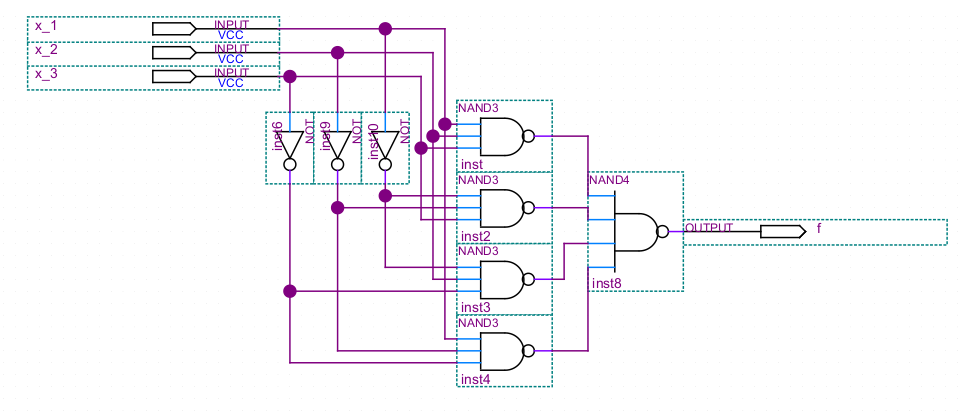
\includegraphics[width=\linewidth]{files/hw2p3.png}

\begin{prob}
 Implement the function in Table~\ref{tab:3-way-light-switch} using only NOR
 gates. [10 marks]
\end{prob}
\subsubsection*{Solution}
{\tiny
\begin{align*}
  f &= (x_1 + x_2 + x_3)(x_1 + \bx_2 + \bx_3)(\bx_1 + x_2 + \bx_3)(\bx_1 + \bx_2 + x_3)
      \\
    &=\overline{\overline{(x_1 + x_2 + x_3)}}\overline{\overline{(x_1 + \bx_2 + \bx_3)}}\overline{\overline{(\bx_1 + x_2 + \bx_3)}}\overline{\overline{(\bx_1 + \bx_2 + x_3)}}
      \\
    &=\overline{\overline{{(x_1 + x_2 + x_3)}} + {\overline{(x_1 + \bx_2 + \bx_3)}} + {\overline{(\bx_1 + x_2 + \bx_3)}} + {\overline{(\bx_1 + \bx_2 + x_3)}}}
\end{align*}
}
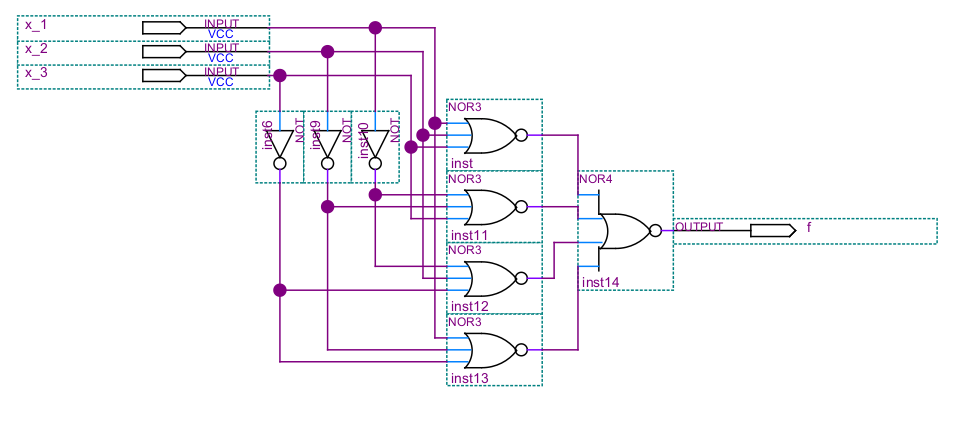
\includegraphics[width=\linewidth]{files/hw2p4.png}

\section{Sept 13th Lecture}

\begin{prob}
Find the minimum-cost SOP and POS forms for the function $f(x_1 , x_2 , x_3 ) =
m(1, 2, 3, 5)$. \cite[Prob 2.37]{brown2013fundamentals} [10 marks]
\label{prob:237}
\end{prob}

\subsubsection*{Solution}

Minimum cost SOP
\\
\begin{tabular}{c|c|c|c|c}
  \toprule
  & \multicolumn{2}{c|}{$\bx_1$} & \multicolumn{2}{c}{$x_1$}
  \\
  & $\bx_2$ & \multicolumn{2}{c|}{$x_2$} & $\bx_2$
  \\ \midrule
  $\bx_3$
                                  & 0 & {\color{red}1} & 0 & 0
  \\
  $x_3$
                                  & {\color{green}1} & {\color{red}1} & 0 & {\color{green}1}
  \\\bottomrule
\end{tabular}.
\\
\begin{align}
  f = {\cred \bx_1 x_2} + {\cg \bx_2 x_3}
\end{align}
Cost = 2 AND  + 1 OR + (2*2 + 2) inputs = 9

Minimum cost POS
\\
\begin{tabular}{c|c|c|c|c}
  \toprule
  & \multicolumn{2}{c|}{$\bx_1$} & \multicolumn{2}{c}{$x_1$}
  \\
  & $\bx_2$ & \multicolumn{2}{c|}{$x_2$} & $\bx_2$
  \\ \midrule
  $\bx_3$
  & \cred 0 & 1 & \cg 0 & \cred 0
  \\
  $x_3$
  & 1 & 1 & \cg 0 & 1
  \\\bottomrule
\end{tabular}.
\\
\begin{align}
  \bar{f} &= {\cred \bx_2 \bx_3} + {\cg x_1 x_2 }
  \\
  \implies f &= {\cred (x_2 + x_3)}{\cg (\bx_1 + \bx_2) }
\end{align}
Cost = 2 OR + 1 AND + (2*2+2) inputs = 9

\begin{prob}
Find the minimum-cost SOP and POS forms for the function $f(x_1 , x_2 , x_3) =
\sum m(1, 4, 7) + D(2, 5)$. \cite[Prob 2.38]{brown2013fundamentals} [10 marks]
\end{prob}

\subsubsection*{Solution}

Minimum cost SOP
\\
\begin{tabular}{c|c|c|c|c}
  \toprule
  & \multicolumn{2}{c|}{$\bx_1$} & \multicolumn{2}{c}{$x_1$}
  \\
  & $\bx_2$ & \multicolumn{2}{c|}{$x_2$} & $\bx_2$
  \\ \midrule
  $\bx_3$
                                  & 0 & d & 0 & \cred 1
  \\
  $x_3$
                                  & \cb 1 & 0 & {\cg 1} & {\cg d} + \cred d + \cb d
  \\\bottomrule
\end{tabular}.
\\
\begin{align}
  f = {\cred x_1 \bx_2} + {\cg x_1 x_3} + {\cb \bx_2 x_3}
\end{align}
Cost = 3 AND  + 1 OR + (3*2 + 3) inputs = 13

Minimum cost POS
\\
\begin{tabular}{c|c|c|c|c}
  \toprule
  & \multicolumn{2}{c|}{$\bx_1$} & \multicolumn{2}{c}{$x_1$}
  \\
  & $\bx_2$ & \multicolumn{2}{c|}{$x_2$} & $\bx_2$
  \\ \midrule
  $\bx_3$
  & \cred 0 & 1 & \cg 0 & \cred 0
  \\
  $x_3$
  & 1 & 1 & \cg 0 & 1
  \\\bottomrule
\end{tabular}.
\\
\begin{align}
  \bar{f} &= {\cred \bx_2 \bx_3} + {\cg x_1 x_2 }
  \\
  \implies f &= {\cred (x_2 + x_3)}{\cg (\bx_1 + \bx_2) }
\end{align}
Cost = 2 OR + 1 AND + (2*2+2) inputs = 9

\begin{prob}
Find the minimum-cost SOP and POS forms for the function $f(x_1 , x_2 , x_3,
x_4) = \prod M(0, 1, 2, 4, 5, 7, 8, 9, 10, 12, 14, 15).$ \cite[Prob
2.39]{brown2013fundamentals} [10 marks]
\end{prob}

\begin{prob}
Find the minimum-cost SOP and POS forms for the function $f(x_1 , x_2 , x_3, x_4) =
\sum m(0, 2, 8, 9, 12, 15) + D(1, 3, 6, 7).$ \cite[Prob
2.40]{brown2013fundamentals} [10 marks]
\end{prob}

\begin{prob}
Derive a minimum-cost realization of the four-variable function that is equal to 1 if exactly
two or exactly three of its variables are equal to 1; otherwise it is equal to
0. \cite[Prob 2.46]{brown2013fundamentals} [10 marks]
\end{prob}

\begin{prob}
  Find the minimum-cost SOP and POS forms for the function $f(x_1 , \dots, x_5) =
  \sum m(0, 1, 3, 4, 6, 8, 9, 11, 13, 14, 16, 19, 20, 21, 22, 24, 25) + D(5, 7,
  12, 15, 17, 23).$  \cite[Prob 2.42]{brown2013fundamentals} [10 marks]
\end{prob}

\bibliography{main}
\bibliographystyle{plain}
\end{document}
